\documentclass{article}
\usepackage{graphicx,psfrag,epsfig,epsf,latexsym,hhline,amsmath,amssymb,multirow,pgfplots}
\usepackage[usenames,dvipsnames]{pstricks}
\usepackage{pst-plot}
\usepackage{pstricks-add}
\usepackage{color}
\usepackage{stmaryrd}
\usepackage{makecell}

\interdisplaylinepenalty=2500
\usepackage{graphicx}
\usepackage{amsthm}
\usepackage{footnote}

\usepackage{blindtext}
\usepackage{etoolbox}

\usepackage{tikz}
\usepackage{pgfplots}
\usepgflibrary{shapes}
\usetikzlibrary{arrows,shapes,chains,matrix,positioning,scopes,patterns	}
\pgfplotsset{compat=newest}
\pgfplotsset{plot coordinates/math parser=false}

\newlength\figureheight 
\newlength\figurewidth

\newcommand{\mc}[1]{\mathcal{#1}}
\newcommand{\ms}[1]{\mathscr{#1}}
\newcommand{\mbb}[1]{\mathbb{#1}}
\newcommand{\mbf}[1]{\mathbf{#1}}
\newcommand{\tit}[1]{\textit{#1}}
\newcommand{\tbf}[1]{\textbf{#1}}
\newcommand{\tsc}[1]{\textsc{#1}}

\newcommand{\defeq}{\triangleq}
\newcommand{\coleq}{\mathrel{\mathop:}=}
\newcommand{\Pp}{\mathbb{P}}
\newcommand{\E}{\mathbb{E}}
\newcommand{\N}{\mathbb{N}}
\newcommand{\Z}{\mathbb{Z}}
\newcommand{\Zp}{\mathbb{Z}_{+}}
\newcommand{\R}{\mathbb{R}}
\newcommand{\Rp}{\R_{+}}
\newcommand{\g}{\mathbf{g}_}
\newcommand{\cp}{\times}
\newcommand{\Lmb}{\Lambda}
\newcommand{\lmb}{\lambda}
\newcommand{\tx}[1]{\text{#1}}

\newcommand{\Q}{\mathbb{Q}}
\newcommand{\F}{\mathbb{F}}
\newcommand{\Zw}{\mathbb{Z}[\omega]}
\newcommand{\Zi}{\mathbb{Z}[i]}
\newcommand{\C}{\mathcal{C}}

\newcommand{\abs}[1]{\lvert{#1}\rvert}
\newcommand{\card}[1]{\abs{#1}}
\newcommand{\norm}[1]{\lVert{#1}\rVert}
\newcommand{\iid}{i.\@i.\@d.\ }

\newcommand{\ceil}[1]{\lceil{#1}\rceil}
\newcommand{\floor}[1]{\lfloor{#1}\rfloor}

\DeclareMathOperator*{\argmax}{arg\,max}
\DeclareMathOperator*{\argmin}{arg\,min}

\theoremstyle{definition}\newtheorem{lemma}{Lemma}
\theoremstyle{definition}\newtheorem{proposition}[lemma]{Proposition}
\theoremstyle{definition}\newtheorem{theorem}[lemma]{Theorem}
\theoremstyle{definition}\newtheorem{corollary}[lemma]{Corollary}
\newtheorem{definition}[lemma]{Definition}
\newtheorem{Example}[lemma]{Example}
\newtheorem{Remark}[lemma]{Remark}
\newtheorem*{Discussion}{Discussion}
%\newtheorem{example}[theorem]{Example}



\newcommand{\ind}{{\rm 1\hspace*{-0.4ex}\rule{0.1ex}{1.52ex}\hspace*{0.2ex}}}
\newcommand{\dbar}[1]{\bar{\bar{#1}}}
\newcommand{\T}{\msf{T}}
\newcommand{\dotleq}{\mathrel{\dot{\leq}}}
\newcommand{\dotgeq}{\mathrel{\dot{\geq}}}
\newcommand{\dotl}{\mathrel{\dot{<}}}
\newcommand{\dotg}{\mathrel{\dot{>}}}
\newcommand{\from}{\colon}

\DeclareMathOperator{\rank}{rank}
\DeclareMathOperator{\tr}{tr}
\DeclareMathOperator{\cl}{cl}
\DeclareMathOperator{\diag}{diag}
\DeclareMathOperator{\conv}{conv}
\DeclareMathOperator{\Bernoulli}{Bernoulli}
\DeclareMathOperator{\Ei}{Ei}
\DeclareMathOperator{\OR}{OR}
\DeclareMathOperator{\Geom}{Geom}
\DeclareMathOperator{\var}{var}
%\setlength\figureheight{4.5cm}
%\setlength\figurewidth{7cm}
\begin{document}
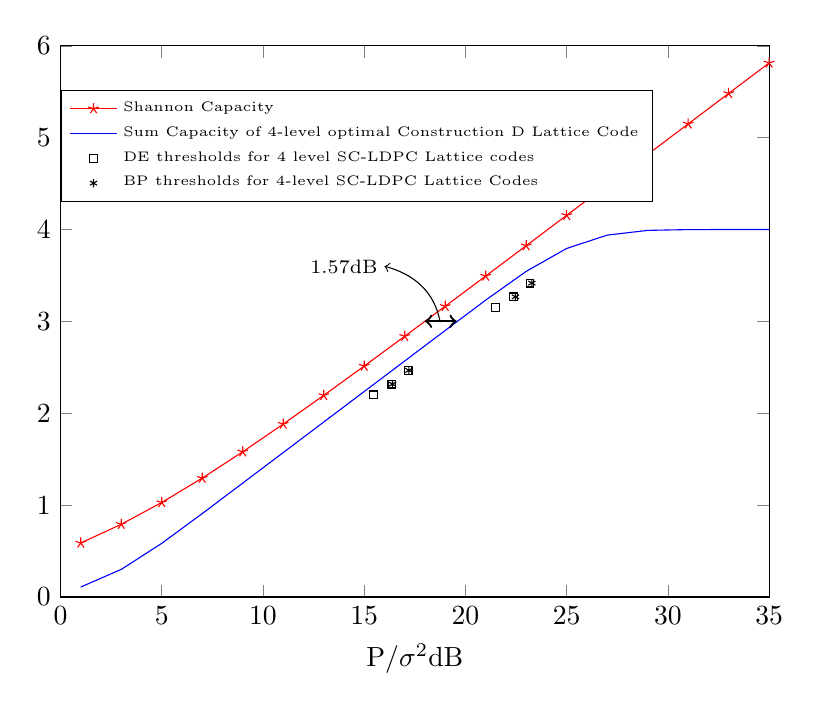
\begin{tikzpicture}
\begin{axis}[
width=9cm,
height=7cm,
scale only axis,
xmin=0,
xmax=35,
xlabel={$\text{P/}\sigma{}^{\text{2}}\text{dB}$},
ymin=0,
ymax=6,
legend style={at={(0,0.717225783363562)},anchor=south west,draw=black,fill=white,legend cell align=left,font=\tiny}
]
\addplot [
color=red,
solid,
mark=star,
mark options={solid}
]
table[row sep=crcr]{
1 0.587818317346194\\
3 0.791341177455778\\
5 1.0286866043034\\
7 1.29390718678102\\
9 1.58040221195651\\
11 1.88219718352143\\
13 2.19452948368152\\
15 2.51390383667526\\
17 2.83788995090244\\
19 3.16485622972095\\
21 3.49373172947796\\
23 3.8238235812452\\
25 4.1546876206064\\
27 4.48604077166048\\
29 4.81770328916082\\
31 5.14956130632863\\
33 5.48154279616551\\
35 5.81360224010802\\
};
\addlegendentry{Shannon Capacity};

\addplot [
color=blue,
solid
]
table[row sep=crcr]{
1 0.108452421861326\\
3 0.30023434461803\\
5 0.583744051972549\\
7 0.908016893863155\\
9 1.23986729393466\\
11 1.57212348172311\\
13 1.90441001540582\\
15 2.23669080702334\\
17 2.56895109146972\\
19 2.90120263165125\\
21 3.23173038940203\\
23 3.54445589072375\\
25 3.7941222586385\\
27 3.93912155348957\\
29 3.99069691963094\\
31 3.99949543839257\\
33 3.99999469407798\\
35 3.99999999597798\\
};
\addlegendentry{Sum Capacity of 4-level optimal Construction D Lattice Code};

\addplot [
color=black,
mark size=1.4pt,
only marks,
mark=square,
]
table[row sep=crcr]{
21.4693 3.15\\
22.3844 3.2667\\
23.1876 3.4167\\
15.4486951388326 2.2\\
16.3638449500461 2.3167\\
17.1669877129645 2.4667\\
};
\addlegendentry{DE thresholds for 4 level SC-LDPC Lattice codes};

\addplot [
color=black,
mark size=1.5pt,
only marks,
mark=asterisk,
mark options={solid},
]
table[row sep=crcr]{
23.2798476914952 3.41666666666667\\
22.4669998480458 3.26666666666667\\
16.3950035382421 2.31666666666667\\
17.2078513816915 2.46666666666667\\
};
\addlegendentry{BP thresholds for 4-level SC-LDPC Lattice Codes};


\draw[<->,thick] (axis cs:18,3.001) -- (axis cs:19.57,3.001);
\draw[->] (axis cs:18.75,2.99) to [out=100,in=345] (axis cs:16,3.6);
\node[font=\scriptsize] at (axis cs:14,3.6){1.57dB};

\end{axis}
\end{tikzpicture}
\end{document} 